% Options for packages loaded elsewhere
\PassOptionsToPackage{unicode}{hyperref}
\PassOptionsToPackage{hyphens}{url}
%
\documentclass[
  english,
  man,floatsintext]{apa6}
\usepackage{lmodern}
\usepackage{amssymb,amsmath}
\usepackage{ifxetex,ifluatex}
\ifnum 0\ifxetex 1\fi\ifluatex 1\fi=0 % if pdftex
  \usepackage[T1]{fontenc}
  \usepackage[utf8]{inputenc}
  \usepackage{textcomp} % provide euro and other symbols
\else % if luatex or xetex
  \usepackage{unicode-math}
  \defaultfontfeatures{Scale=MatchLowercase}
  \defaultfontfeatures[\rmfamily]{Ligatures=TeX,Scale=1}
\fi
% Use upquote if available, for straight quotes in verbatim environments
\IfFileExists{upquote.sty}{\usepackage{upquote}}{}
\IfFileExists{microtype.sty}{% use microtype if available
  \usepackage[]{microtype}
  \UseMicrotypeSet[protrusion]{basicmath} % disable protrusion for tt fonts
}{}
\makeatletter
\@ifundefined{KOMAClassName}{% if non-KOMA class
  \IfFileExists{parskip.sty}{%
    \usepackage{parskip}
  }{% else
    \setlength{\parindent}{0pt}
    \setlength{\parskip}{6pt plus 2pt minus 1pt}}
}{% if KOMA class
  \KOMAoptions{parskip=half}}
\makeatother
\usepackage{xcolor}
\IfFileExists{xurl.sty}{\usepackage{xurl}}{} % add URL line breaks if available
\IfFileExists{bookmark.sty}{\usepackage{bookmark}}{\usepackage{hyperref}}
\hypersetup{
  pdftitle={Phonological Networks and Systematicity in Early Lexical Acquisition},
  pdfauthor={Catherine E. Laing1},
  pdflang={en-EN},
  pdfkeywords={Systematicity, Phonological development, preferential attachment, networks analysis},
  hidelinks,
  pdfcreator={LaTeX via pandoc}}
\urlstyle{same} % disable monospaced font for URLs
\usepackage{graphicx,grffile}
\makeatletter
\def\maxwidth{\ifdim\Gin@nat@width>\linewidth\linewidth\else\Gin@nat@width\fi}
\def\maxheight{\ifdim\Gin@nat@height>\textheight\textheight\else\Gin@nat@height\fi}
\makeatother
% Scale images if necessary, so that they will not overflow the page
% margins by default, and it is still possible to overwrite the defaults
% using explicit options in \includegraphics[width, height, ...]{}
\setkeys{Gin}{width=\maxwidth,height=\maxheight,keepaspectratio}
% Set default figure placement to htbp
\makeatletter
\def\fps@figure{htbp}
\makeatother
\setlength{\emergencystretch}{3em} % prevent overfull lines
\providecommand{\tightlist}{%
  \setlength{\itemsep}{0pt}\setlength{\parskip}{0pt}}
\setcounter{secnumdepth}{-\maxdimen} % remove section numbering
% Make \paragraph and \subparagraph free-standing
\ifx\paragraph\undefined\else
  \let\oldparagraph\paragraph
  \renewcommand{\paragraph}[1]{\oldparagraph{#1}\mbox{}}
\fi
\ifx\subparagraph\undefined\else
  \let\oldsubparagraph\subparagraph
  \renewcommand{\subparagraph}[1]{\oldsubparagraph{#1}\mbox{}}
\fi
% Manuscript styling
\usepackage{upgreek}
\captionsetup{font=singlespacing,justification=justified}

% Table formatting
\usepackage{longtable}
\usepackage{lscape}
% \usepackage[counterclockwise]{rotating}   % Landscape page setup for large tables
\usepackage{multirow}		% Table styling
\usepackage{tabularx}		% Control Column width
\usepackage[flushleft]{threeparttable}	% Allows for three part tables with a specified notes section
\usepackage{threeparttablex}            % Lets threeparttable work with longtable

% Create new environments so endfloat can handle them
% \newenvironment{ltable}
%   {\begin{landscape}\centering\begin{threeparttable}}
%   {\end{threeparttable}\end{landscape}}
\newenvironment{lltable}{\begin{landscape}\centering\begin{ThreePartTable}}{\end{ThreePartTable}\end{landscape}}

% Enables adjusting longtable caption width to table width
% Solution found at http://golatex.de/longtable-mit-caption-so-breit-wie-die-tabelle-t15767.html
\makeatletter
\newcommand\LastLTentrywidth{1em}
\newlength\longtablewidth
\setlength{\longtablewidth}{1in}
\newcommand{\getlongtablewidth}{\begingroup \ifcsname LT@\roman{LT@tables}\endcsname \global\longtablewidth=0pt \renewcommand{\LT@entry}[2]{\global\advance\longtablewidth by ##2\relax\gdef\LastLTentrywidth{##2}}\@nameuse{LT@\roman{LT@tables}} \fi \endgroup}

% \setlength{\parindent}{0.5in}
% \setlength{\parskip}{0pt plus 0pt minus 0pt}

% \usepackage{etoolbox}
\makeatletter
\patchcmd{\HyOrg@maketitle}
  {\section{\normalfont\normalsize\abstractname}}
  {\section*{\normalfont\normalsize\abstractname}}
  {}{\typeout{Failed to patch abstract.}}
\patchcmd{\HyOrg@maketitle}
  {\section{\protect\normalfont{\@title}}}
  {\section*{\protect\normalfont{\@title}}}
  {}{\typeout{Failed to patch title.}}
\makeatother
\shorttitle{Systematicity in early phonological development}
\keywords{Systematicity, Phonological development, preferential attachment, networks analysis}
\usepackage{lineno}

\linenumbers
\usepackage{csquotes}
\DeclareDelayedFloatFlavor{kableExtra}{table}
\usepackage{tipa}
\ifxetex
  % Load polyglossia as late as possible: uses bidi with RTL langages (e.g. Hebrew, Arabic)
  \usepackage{polyglossia}
  \setmainlanguage[]{english}
\else
  \usepackage[shorthands=off,main=english]{babel}
\fi

\title{Phonological Networks and Systematicity in Early Lexical Acquisition}
\author{Catherine E. Laing\textsuperscript{1}}
\date{}


\affiliation{\vspace{0.5cm}\textsuperscript{1} University of York, York, UK}

\abstract{
Early on in lexical acquisition, infants' words tend to be phonologically similar to one another. This may reflect a systematic approach to early production, as infants draw on `whole word' structures (cf.~Vihman, 2014, 2019), whereby they adapt newly-acquired forms to fit their existing production patterns. This reflects a `rich-get-richer' approach to phonological acquisition, also known as \emph{preferential attachment} in network science, where new words are acquired that are similar to (and therefore connect to) existing highly-connected words in the lexicon (or network). This contrasts with recent network analyses of lexical acquisition (Fourtassi et al., 2020) showing that the learning environment is the key predictor in learning (i.e.~\emph{preferential acquisition}). However, previous studies of network growth in early word learning have drawn on norming data taken from thousands of children, which does not capture the expected variability in early phonological development. In this study, phonetic transcriptions of nine infants' word productions were analysed from word onset to age 2;6. Network growth models were generated for each participant to test whether acquisition was best modelled through preferential attachment or preferential aquisition. Results show that both models of growth can explain early acquistion, but the preferential attachment model was more convincing across the board. This suggests that infants' early words are systematically acquired according to their phonological properties, such that newly-acquired words are phonologically similar to existing words in the network. This approach may help infants address the challenges of word production in early development, when memory, planning and articulatory capacity are simultaneously limited.
}



\begin{document}
\maketitle

A wide body of literature spanning decades of work on phonological development has documented the systematic nature of infants' earliest words. Studies of phonetic (McCune \& Vihman, 2001) and phonological structures (Vihman, 2016) show that many of a child's first word forms share similar properties. Infants appear to draw on what they know: when articulatory, memory and planning capacities are simultaneously limited in early development, infants draw on a \enquote{phonic core of remembered lexical items and articulations} (Ferguson \& Farwell, 1975, p. 112) in order to deal with the challenges involved in developing an early lexicon. Vihman (2019, p. 263) describes early word acquisition as \enquote{an emergent network of related forms} that reveals an inherent systematicity in infants' early-established lexicon. A networks approach to phonological development offers one way of tracing developing systematicity in infants' early forms. In this study, I present a longitudinal analysis of lexical development across nine infants to identify systematicity in the first three years of word production. I consider the phonological characteristics of the developing lexicon using network analysis to demonstrate how early systematicity may be integral to the developing linguistic system, supporting infants to acquire the requisite capacity for flexible, automatic and target-like word production.

Waterson (1971) was the first to observe systematic output patterns in early production. In a case study of her son's early words, she noted striking systematicity in his lexicon at 18 months. She details a number of systematic structures, or \enquote{schema}, that share common segments and features. For example, he systematically adapts /n/-medial forms including \emph{finger}, \emph{window} and \emph{another} to a reduplicated schema with a palatal nasal stop at syllable onset, {[}\textipa{\*n}V\textipa{\*n}V{]}. Waterson posits that schemas come about through the child's perception of salient features in the adult form, which, crucially, are already in the child's own productive repertoire. According to Waterson, schemas relate holistically to the adult target (see also Vihman, 2019), based on salient and reproducible features of the input form.

Since Waterson's landmark study, a rich body of work has developed with the aim of identifying systematic schemas in infants' early words. Most notably, Vihman's (2014, 2019) work on phonological templates has brought together a wide body of evidence to present a compelling theory of early phonological development. In Vihman's model, the child begins with a small lexicon of phonologically-simple and accurately-produced forms. In this sense, early words tend to look similar across children, with some evidence of ambient language effects (Boysson-Bardies \& Vihman, 1991). Vihman proposes that these early words are \enquote{selected} for their ease of production, as well as their perceptual salience. At first, new words are \enquote{selected} to fit these familiar patterns, but as the lexicon grows, target forms that do not necessarily fit these structures are \enquote{adapted} so that they do. Selection and, later, adaption indicate the presence of systematicity within the developing lexicon. The constraints on infants' production are high - whether for reasons of articulation, memory, planning, perception, or a combination of these - and so they draw on a limited set of vocal outputs that represent a growing number of target words. Essentially, the new target form is allocated to one of a small number of motoric categories, and as these categories increase in size they become further entrenched. For example, in data from their bilingual (English-Spanish) daughter's early word acquisition, Deuchar and Quay (2000) show that 13 of her first 20 words are produced with a CV structure, and many are phonologically identical: she produces \emph{car}, \emph{clock}, \emph{casa} \enquote{house} and \emph{cat} as /ka/, and \emph{papa} \enquote{daddy}, \emph{pájaro} \enquote{bird} and \emph{panda} as /pa/.

One way of interrogating phonological systematicity in early phonological productions is through network analysis, which offers a quantitative perspective on the organization and development of the lexicon. Developmental research in this area centres around the words that children target in production to establish connectivity on phonological (e.g.~Siew \& Vitevitch, 2020) and semantic (e.g.~Hills, Maouene, Maouene, Sheya, \& Smith, 2009) planes - that is, how similar pairs of target words are to one another in form or meaning, and what this might mean for acquisition. However, as yet there is no work looking at the way children produce those words; that is, whether or not children are drawing on systematicity in the output. In this context, the term \emph{network} refers to a web of forms (or \emph{nodes}, in network terms) that are interconnected based on shared properties. Here these are phonological properties, but could also be semantic, or indeed non-linguistic properties such as genetic information, social connections or location (see Bell et al., 2017, for a review). Network growth models allow analysis of changes within a system over time, and two key models\footnote{A third model - Lure of the Associates - has also been considered in some studies (Hills et al., 2009; Siew \& Vitevitch, 2020) but will not be considered here.} of development have been proposed for lexical acquisition: preferential attachment (hereafter \textbf{PAT}) and preferential acquisition (hereafter \textbf{PAQ}; Hills et al., 2009; see also Steyvers \& Tenenbaum, 2005a). PAT models of network growth propose a rich-get-richer scenario, whereby the most highly-connected nodes (nodes with more \emph{edges}) in the network attract new nodes at any given time-point. In phonological development terms, this model implies that the lexicon will constitute clusters of similar-sounding words, and that a child is more likely to acquire new words that attach to these dense clusters: infants' production of newly-acquired words will be similar to their production of existing words in the lexicon. PAT-like growth is therefore driven by the \emph{internal} linguistic system. On the other hand, PAQ-like growth assumes that forms in the learning environment that connect to (i.e.~share properties with) a higher number of \emph{different} nodes in the existing network will be acquired first. PAQ models of network growth thus assume that \emph{external} factors in the learning environment influence acquisition - that is, words that are well-connected to one another within the target language will be acquired earlier. In phonological terms, this would mean that early productions would constitute a more even distribution of segments and structures, resembling the statistical properties of the ambient language more closely, rather than a \enquote{pattern force} driven by dominant segments and structures in the existing lexicon.

A number of studies have drawn on network growth models to test whether PAT- and PAQ-like growth\footnote{Note that these are not mutually exclusive.} can explain lexical development in semantic and phonological networks of acquisition. Hills and colleagues' (2009) study of semantic networks showed evidence for PAQ, but not PAT, in associative networks of normed vocabulary acquisition data. Amatuni and Bergelson (2017) support this evidence for PAQ-like growth in semantic networks with an analysis of a large-scale corpus of input data, combined with normed productive vocabulary data derived from WordBank (Frank, Braginsky, Yurovsky, \& Marchman, 2017). More recent work has applied these same approaches to phonological data: Fourtassi, Bian and Frank (2020) analyse both phonological and semantic network growth from vocabulary norms (receptive and productive) in 10 languages to find consistent evidence in support of PAQ-like growth, for both phonological and semantic networks, receptive and productive vocabularies, and across the 10 languages included in their analysis. In contrast, Siew and Vitevitch (2020) tested phonological networks in acquisition of older Dutch- and English-learning children (age 3-9 years), again using vocabulary norms to indicate age of acquisition for each word. Their analysis revealed contrasting findings for English compared with Dutch, as well as an age effect: PAT-like network growth predicted acquisition in English but not Dutch, whereas both PAT and PAQ (as well as a third model, Lure of the Associates, not discussed here) predicted word learning in Dutch. Regarding the effect of age, PAT was a better predictor of acquisition earlier on in development (i.e.~newly-acquired words were likely to attach to densely-connected clusters of similar forms); later on, the opposite was found, whereby later-acquired words tended to be phonologically more distinct (i.e.~newly-acquired words were less similar to existing words in the network).

Together these studies present an intersection of evidence for the role of PAT and PAQ network growth in phonological development. However, there are two key aspects of the existing approaches that should be expanded further. First, the consideration of acquisition in terms of only target forms provides no view of systematicity in \emph{production}, which is where systematicity has been most well-documented in naturalistic data. Second, vocabulary norming data abstracts away from the individual differences expected in early phonological development (e.g.~Vihman, Kay, Boysson-Bardies, Durand, \& Sundberg, 1994); by drawing on data that generalises across hundreds of different children, it may not be possible to gain a realistic picture of a developing phonological network in the individual, thus making it difficult to test which model of network growth (PAT or PAQ) is most cogent. To better understand the role of systematicity in early word production, it is essential to consider infants' \emph{actual productions} of their early word forms, in terms of both \emph{how} and \emph{when} they produce them. In this paper, I analyse phonological networks of both \emph{target} and \emph{actual forms} (that is, the words children produce, and the way they produce them) produced in naturalistic data from two languages, in order to consider systematicity in early production within the individual development trajectories of nine infants.

\hypertarget{hypotheses}{%
\section{Hypotheses}\label{hypotheses}}

Drawing on naturalistic data, this study will use network growth models to capture the phonological connectivity (taken here as an index here of systematicity) within the individual lexicons of nine infants. By drawing on corpus data, the analysis will take into account the individual variability that is observed in models of early development (Vihman, 1993), which is not possible to capture in normed vocabulary data. Two sets of networks will be established for each infant: one tracing connections between infants' \emph{actual} word productions, the other between the \emph{target} productions of these forms. Network analysis will quantify systematicity in the developing lexicon via two key network growth frameworks: PAT and PAQ. I will draw on approaches outlined in previous studies (Amatuni \& Bergelson, 2017; Fourtassi et al., 2020; Siew \& Vitevitch, 2020) to test whether naturalistic data of infants' actual productions reveals evidence of systematicity in infants' output forms, such that language development is shaped by infants' existing production knowledge. Specifically, I predict that:

H1) Early phonological networks will show stronger evidence of a PAT-like model of growth over a PAQ-like model, based on evidence from the phonological development literature that shows similarity across individual infants' developing lexicons (e.g.~Vihman \& Keren-Portnoy, 2013).

H2) PAT-like growth will be most evident earlier on in development, as infants select and then adapt words to fit their production capacity (Vihman, 2019). Later, more variability (i.e.~fewer clusters of similar words) is expected as phonological capacity develops.

H3) If PAT-like growth is supported in the data, then this should be more convincing for Actual than Target productions, given that we expect infants to adapt target words to fit the motor routines that are most accessible to them in production. This difference is not expected for a PAQ-like model of network growth, which assumes that network growth reflects connectivity in the input; PAQ thus assumes that Actual and Target networks do not differ.

To test these hypotheses, individual phonological networks will be established for nine infants acquiring American English or French. Phonological distance will be calculated between each word and each other word in each infant's network to establish connectivity within the network. Logistic regression models will determine whether acquisition of \emph{Actual} and \emph{Target} forms reflects PAT- or PAQ-like growth in early phonological development.

\hypertarget{methods}{%
\section{Methods}\label{methods}}

This analysis follows approaches taken by Hills and colleagues (2009) and Siew and Vitevitch (2020), by establishing network growth values for each word in each child's lexicon. This is followed up by drawing on approaches taken by Amatuni and Bergelson (2017), using simulated data to analyse network properties (see below).

\hypertarget{data-and-materials}{%
\subsection{Data and Materials}\label{data-and-materials}}

Data for this study were extracted from CHILDES (Child Language Data Exchange System, MacWhinney, 2000) using Phon (Hedlund \& Rose, 2020). Two corpora were selected for the analysis: American English (Providence corpus, Demuth, Culbertson, \& Alter, 2006) and French (Lyon corpus, Demuth \& Tremblay, 2008). These corpora were selected due to their parallel data collection and transcription methods. The English data includes five infants (including two boys\footnote{The Providence corpus (Demuth et al., 2006) includes six children and three boys. One child was later diagnosed with Asperger's syndrome, and so is omitted from this analysis. The Lyon corpus (Demuth \& Tremblay, 2008) includes five children (two boys) but one of the datasets (Marilyn) is not fully transcribed and is therefore excluded from this analysis.}) and four infants from the French corpus (two boys). Both corpora include spontaneous interactions between child and caregiver, recorded in the home for one hour every two weeks from the onset of first words. The corpora were orthographically transcribed, and then phonetically transcribed and checked by trained coders. See Demuth et al.~(2006) and Demuth and Tremblay (2008) for full details of data collection and annotation.

For the purposes of this analysis, transcripts were extracted from the first session in the dataset (the first session in which the child produced a word) until the final session taken at age 2;6. Words produced in each month were aggregated to give a rolling monthly network of all words produced by each child; the first instance of each word type (i.e.~every unique word: \emph{bring} and \emph{bringing} were considered as unique words, though plurals were categorised with their singular nouns; see Jones \& Brandt, 2019) in each child's full dataset was considered as the first production of that word, and was included in that month's list of newly-acquired words. Later productions of the same word were not included in the dataset. Two of the American infants (Naima and Lily) are reported to have denser data taken at weekly intervals during some periods of data collection, but this is not considered to be an issue for the purposes of this analysis as no between-child comparisons will be conducted. The total network of words at any given month amounts to all the words produced up to and including that month. The phonetic transcription of each word produced by each infant in each session was extracted (\emph{Actual} forms, i.e., the phonological form as produced by the child) alongside its target transcription (\emph{Target} forms). For both Actual and Target forms, phonological distance was calculated between every word and every other word in the cumulative network at each month, following Monaghan, Christiansen, Farmer and Fitneva's (2010) approach. This is based on phonological features, following Harm and Seidenberg (1999) and based on Chomsky and Halle's (1968) theory of government phonology. This was considered to be the most appropriate measure of phonological distance, as oppose to other established measures such as Levenshtein distance (e.g.~Fourtassi et al., 2020; Siew \& Vitevitch, 2020): distinctive features allow us to consider distance on a phonologically-appropriate gradient, whereby the difference between words such as \emph{bat} and \emph{pat} is smaller than the difference between \emph{bat} and \emph{rat}. Using edit distance as a measure, \emph{pat}, \emph{bat} and \emph{rat} would be equidistant, thereby equating all phonemes as articulatorily similar, which does not reflect the realities of phonological development (cf.~McLeod \& Crowe, 2018).

Only words included on the US English and French communicative development inventories (CDIs, Fenson et al., 1994; Kern \& Gayraud, 2010) were analysed. The final dataset includes 2745 word types, aggregated across infants (English=, French=). See Table \ref{tab:table-data-overview} for a breakdown by corpus and child.

\begin{longtable}[t]{ccccc}
\caption{\label{tab:table-data-overview}Minimum age, number of sessions and number of distinct word types produced by each child in the dataset - an index of each child's global network size. Means and SDs for each corpus are shown in the bottom four rows of the table.}\\
\toprule
Speaker & Corpus & Min. age & n Sessions & Types\\
\midrule
Alex & English & 16 & 14 & 276\\
Lily & English & 13 & 16 & 498\\
Naima & English & 11 & 19 & 468\\
Violet & English & 14 & 14 & 409\\
\midrule
\textbf{William} & \textbf{English} & \textbf{16} & \textbf{13} & \textbf{280}\\
\addlinespace
\textbf{Mean} & \textbf{English} & \textbf{14} & \textbf{15} & \textbf{386}\\
\midrule
SD & English & 2 & 2 & 104\\
Anais & French & 14 & 15 & 202\\
Marie & French & 12 & 14 & 184\\
Nathan & French & 12 & 16 & 121\\
\addlinespace
Tim & French & 12 & 16 & 307\\
\midrule
\textbf{Mean} & \textbf{French} & \textbf{12} & \textbf{15} & \textbf{204}\\
\textbf{SD} & \textbf{French} & \textbf{1} & \textbf{1} & \textbf{77}\\
\midrule
\textbf{Mean} & \textbf{All} & \textbf{13} & \textbf{15} & \textbf{305}\\
\textbf{SD} & \textbf{All} & \textbf{2} & \textbf{2} & \textbf{130}\\
\bottomrule
\end{longtable}

\hypertarget{network-analysis}{%
\subsection{Network Analysis}\label{network-analysis}}

For each child, two kinds of network were generated: 1) a \emph{global network}, which represents the final network, i.e.~all words produced in the data by 2;6. This network includes the Target production of all individual word types produced in the dataset, coded for age of first production. The global network is taken to reflect the learning environment, or the input, which is why only Target forms are included; this will be used to establish PAQ growth values for each word in the data (see below), and also serves as a proxy for the \enquote{end-state} towards which each child's phonological development is directed. 2) A series of \enquote{known} networks representing the lexicon at each month; each monthly known network includes all the words produced upto and including the given month, in either Actual (the infants' realization) or Target (the target realization) form. This series of networks is used to generate PAT values for each word in the data. For both kinds of networks, a given word type was included from the first session in which it occurred. When multiple instances of the same word were produced in a single session (i.e.~which might differ from each other phonologically in the child's production), the child's first production of that word was included in the analysis. One important consideration was how to index connectivity within a network: how phonologically similar should two nodes be in order to form an edge? In this study, two nodes were considered to be connected (i.e., formed an edge) if they had a scaled phonological distance lower than 0.25; this value was selected in order to capture the lower quartile of connectivity within the data.

Once networks were established, PAT and PAQ values were calculated for each word. Following Siew and Vitevitch's (2020) approach, these values were generated by computing, for each month, the likelihood that an as-yet-unknown word would form an edge with known words in the existing network (i.e.~the words produced upto and including a given month). The PAT value of a given yet-to-be-learned word represents the mean degree of all the words it would connect to (i.e.~the words that have a phonological distance of 0.25 or less) if it were learned in the following month. For example, a word with a PAT value of 5.6 would connect to a set of words in the following month that, on average, connected to 5.6 other words each. Given that PAT assumes that newly-acquired words will connect to already-well-connected words in the existing network, higher PAT values predict learning (i.e.~new words will connect to words with higher mean degrees). PAT networks were generated with both Actual and Target forms. PAQ values reflect the degree of a given word in the global network (i.e., all words in a given infant's dataset at 2;6). So a word with a PAQ value of 87 would connect to 87 other words in the global network. Again, as PAQ predicts that well-connected words in the global network would be acquired earlier, higher PAQ values predict earlier learning; in each month, we would expect that words with the highest PAQ values will be acquired in the following month. As PAQ-like growth is assumed to represent the learning environment - that is, the connectivity of words in the ambient language - global networks were established with Target forms only. Note that, as both PAT and PAQ values are established through connectivity in the network (i.e.~only words that form an edge with another word are represented), not all words are included in the analysis, as some words did not connect to any other word at a threshold of 0.25.

\hypertarget{data-analysis}{%
\subsection{Data Analysis}\label{data-analysis}}

The data were analysed following previous approaches: network growth models (Fourtassi et al., 2020; Siew \& Vitevitch, 2020; following Hills et al., 2009) simulated networks (Amatuni \& Bergelson, 2017).

\hypertarget{network-growth-models}{%
\subsubsection{Network growth models}\label{network-growth-models}}

Network growth models are logistic regression models that predict whether or not a word was learned in the following month. Here, the binary dependent variable was 1 if the word was learned in the following month, and 0 if it was not. The key predictors of acquisition were PAT/PAQ growth values for each word at each month - the models test the assumption that higher growth values predict learning in the following month. Included in the model as additional fixed effects were frequency of each word in the mothers' input from the respective CHILDES corpus, and word length in phonemes (all variables scaled and centred), as well as age of first production in the child's data (AoP). Subject was included as a random effect with a by-subject random slope for the effect of AoP. Model outputs were generated using model comparisons comparing the model with the variable in question against a null model without the given variable. The English and French data were always modeled separately, as were Target and Actual data, unless otherwise specified. Analysis of Target data includes PAT values for the Target networks, and analysis of Actual data includes PAT values for the Actual networks. PAQ values always represent the Target network only (i.e.~the adult production of a given word in the input).

\hypertarget{simulated-networks}{%
\subsubsection{Simulated networks}\label{simulated-networks}}

PAT-like networks should exhibit properties of small-world network growth - namely a low mean path length and a high clustering coefficient (Amaral, Scala, Barthelemy, \& Stanley, 2011; Steyvers \& Tenenbaum, 2005b; Watts \& Strogatz, 1998): words should be more densely connected, with shorter connections between words, especially in earlier development. To test this, mean path length and clustering coefficient values were generated for both the Target and Actual networks, as outlined below. If these variables change in a PAT-like growth trajectory, then we would expect to see no statistical difference between the network being tested and a simulated small-world network of comparable size (note that it is not possible to draw any conclusions about PAQ-like growth with this approach). Data were compared to the growth of a simulated small-world network, known as a Watts-Strogatz network (Watts \& Strogatz, 1998); if no differences are observed between the real and simulated data over the trajectory of development, then a PAT-like model of network growth may be present in the data. The real data were also compared to a similarly-sized but randomly-generated network known as a Erdős--Rényi model. If the real network grows in a systematic way, then we would expect the real data to differ significantly from the randomly-generated Erdős--Rényi network. To run these analyses, network graphs were computed for each child at each month in the dataset, such that the network grew cumulatively over time - all words produced in the given month and all previous months were included in each month's network. Mean path length and clustering coefficient were calculated for each graph, and then compared to the two kinds of simulated data, matched for network size: a Watts-Strogatz network (prototypical PAT-like network) and an Erdős--Rényi network (random network).

\hypertarget{results}{%
\section{Results}\label{results}}

\hypertarget{age-of-production-aop-connectivity}{%
\subsubsection{Age of production (AoP) \textasciitilde{} connectivity}\label{age-of-production-aop-connectivity}}

As a first step in the analysis, correlations were generated between connectivity and age of first production (hereafter AoP). According to both PAT- and PAQ-like network growth, we would expect words acquired earlier in development to have higher connectivity, or higher degree, in the network. To test this, correlations were generated between the degree of each node in each child's global network, for both Actual and Target forms, and the AoP of that word in the data. Across all infants, there was a mean correlation of \emph{r}=-0.18 (Spearman's, \emph{SD}=0.07), with much stronger correlations observed in the English corpus (mean \emph{r}=-0.23, \emph{SD} =0.03) than the French corpus (mean \emph{r}=-0.13, \emph{SD}=0.06). Significant negative correlations were found in all children's data except Anais (French). See Table S1 and Figure S1.

\hypertarget{network-growth-models-1}{%
\subsubsection{Network growth models}\label{network-growth-models-1}}

Next, network growth models were generated to test whether PAT and PAQ values predicted which words were produced in the following month. For both PAT and PAQ, higher values should predict earlier production, such that, in each month, the as-yet-unknown words with the highest PAT/PAQ values should be learned in the following month. If the models successfully predict which words were acquired, this would indicate that the infants' early phonological networks are developing according to PAT- and/or PAQ-like growth.

All reported models were generated in R (R Core Team, 2020). P-values were established through nested model comparisons. Logistic mixed effects regression models included a binomial dependent variable (coded as 0 or 1) indexing whether, for each as-yet-unknown word at month \emph{n}, it was acquired in month \emph{n+1}. As well as PAT and PAQ growth values, each model included target word length in phonemes, the word's frequency in mothers' speech in the corpus, and age as fixed effects. Infant was specified as a random effect, with a by-subject random slope for the effect of age. All relevant variables were scaled and centred.

Following the approach taken by Siew and Vitevitch (2020), the first step was to construct three models: a null model (model 0) with word length, frequency, and age included as predictors of word learning, and then two additional models with PAT (model 1) and PAQ (model 2) growth values included as predictors, respectively. In each case interactions were included between Word length x Age, Word frequency x Age and PAT/PAQ values x Age. Models 1 and 2 were then compared against model 0 to test for the effects of PAT and PAQ values individually. A third model (model 3) was then constructed that included both PAT and PAQ values as predictors. Data type (Actual and Target) and corpus (English and French) were modeled separately in each case.

\begin{longtable}[t]{ccccccccc}
\caption{\label{tab:table-data-summary-providence}Results from maximal logistic regression models with network growth values, word frequency and word length to predict word acquisition in the English data. All variables were scaled and centred.}\\
\toprule
\multicolumn{1}{c}{ } & \multicolumn{4}{c}{Actual} & \multicolumn{4}{c}{Target} \\
\cmidrule(l{3pt}r{3pt}){2-5} \cmidrule(l{3pt}r{3pt}){6-9}
Effect & beta & SE & z & p & beta & SE & z & p\\
\midrule
Intercept & -2.21 & 0.19 & -11.44 & <0.001 & -2.23 & 0.20 & -11.07 & <0.001\\
Length & -0.19 & 0.04 & -4.24 & <0.001 & -0.21 & 0.05 & -4.52 & <0.001\\
Age & 0.75 & 0.16 & 4.57 & <0.001 & 0.79 & 0.17 & 4.73 & <0.001\\
Word frequency & 0.36 & 0.04 & 10.00 & <0.001 & 0.36 & 0.04 & 9.91 & <0.001\\
PAQ value & 0.04 & 0.04 & 0.94 & 0.349 & 0.05 & 0.04 & 1.20 & 0.231\\
\addlinespace
PAT value & 0.23 & 0.05 & 4.83 & <0.001 & 0.20 & 0.05 & 3.86 & <0.001\\
Age x Length & 0.07 & 0.04 & 1.88 & 0.060 & 0.09 & 0.04 & 2.23 & 0.025\\
Age x Frequency & 0.23 & 0.04 & 5.54 & <0.001 & 0.24 & 0.04 & 5.60 & <0.001\\
Age x PAQ & -0.04 & 0.04 & -1.11 & 0.269 & -0.03 & 0.04 & -0.77 & 0.440\\
Age x PAT & 0.03 & 0.03 & 0.96 & 0.336 & 0.04 & 0.03 & 1.34 & 0.181\\
\bottomrule
\end{longtable}

\begin{longtable}[t]{ccccccccc}
\caption{\label{tab:table-data-summary-lyon}Results from maximal logistic regression models with network growth values, word frequency and word length to predict word acquisition in the French data.}\\
\toprule
\multicolumn{1}{c}{ } & \multicolumn{4}{c}{Actual} & \multicolumn{4}{c}{Target} \\
\cmidrule(l{3pt}r{3pt}){2-5} \cmidrule(l{3pt}r{3pt}){6-9}
Effect & beta & SE & z & p & beta & SE & z & p\\
\midrule
Intercept & -3.14 & 0.09 & -36.49 & <0.001 & -3.45 & 0.15 & -22.93 & <0.001\\
Length & -0.48 & 0.11 & -4.16 & <0.001 & -0.54 & 0.13 & -4.31 & <0.001\\
Age & 1.24 & 0.13 & 9.31 & <0.001 & 1.75 & 0.16 & 11.30 & <0.001\\
Word frequency & 0.14 & 0.05 & 3.17 & 0.002 & 0.14 & 0.05 & 3.14 & 0.002\\
PAQ value & -0.28 & 0.11 & -2.51 & 0.012 & -0.24 & 0.12 & -1.95 & 0.051\\
\addlinespace
PAT value & -0.18 & 0.11 & -1.56 & 0.120 & -0.55 & 0.13 & -4.18 & <0.001\\
Age x Length & 0.38 & 0.09 & 4.07 & <0.001 & 0.45 & 0.10 & 4.51 & <0.001\\
Age x Frequency & -0.08 & 0.04 & -1.84 & 0.066 & -0.07 & 0.04 & -1.66 & 0.097\\
Age x PAQ & 0.24 & 0.09 & 2.71 & 0.007 & 0.22 & 0.10 & 2.33 & 0.020\\
Age x PAT & 0.31 & 0.05 & 5.71 & <0.001 & 0.43 & 0.07 & 6.22 & <0.001\\
\bottomrule
\end{longtable}

As shown in Table \ref{tab:table-model-summary-providence}, PAT, but not PAQ, values improved model fit over and above the effects of word frequency, word length and age for both Actual and Target forms in the English data. A model with both PAT and PAQ values included did not significantly improve model fit over and above a model that only included PAT values. In the French data, both PAT and PAQ values improved model fit for both Actual and Target forms, such that the model with both PAT and PAQ values included proved to be the best fit to the data. See Table \ref{tab:table-model-summary-lyon}. This lends tentative support for H1, in that PAT values predicted acquisition in both datasets. Results suggest that PAQ also plays a role in phonological development.

Model outputs are shown in Tables \ref{tab:table-data-summary-providence} and \ref{tab:table-data-summary-lyon}. Word length, word frequency and age had a significant effect on acquisition across all the data. As we would expect, longer words were acquired later, and more frequent words earlier. Age was a significant predictor of acquisition, likely because over time, as-yet-unknown words are increasingly likely to be learned in the following month. Looking now at the growth values, words with higher PAT values were more likely to be acquired in the English data, and this effect was slightly stronger for Actual (\emph{b}=0.23, \emph{p} \textless{} .001) over Target forms (\emph{b}=0.20, \emph{p} \textless{} .001), again supporting H1, with initial support for H3. In the French corpus, results were less clear in relation to H1: \emph{lower} PAQ values predicted acquisition in the Actual data (\emph{b}=-0.28, \emph{p}=.012), as well as in the Target data, though here the individual contribution of PAQ was only marginally significant (\emph{b}=-0.24, \emph{p}=.051). PAT values were only significant in the Target data, and again \emph{lower} values predicted acquisition (\emph{b}=-0.55, \emph{p} \textless{} .001).

A number of these main effects were qualified by a significant interaction with Age. In the English corpus, word length and frequency interacted significantly with Age in the Actual data, and word frequency also in the Target data. See Table \ref{tab:table-data-summary-providence}. In the French corpus, word length and both PAT and PAQ values interacted with Age in both Actual and Target data. See Table \ref{tab:table-data-summary-lyon}. These interactions will be explored in more detail below.

\hypertarget{interactions}{%
\subsubsection{Interactions}\label{interactions}}

\begin{longtable}[t]{lccccccc}
\caption{\label{tab:table-all-slopes}Simple slopes analyses taken at the mean and ±1SD around the mean scaled age in the dataset for each signficiant interaction in the logistic regression models in the English and French data. All values are z-scored.}\\
\toprule
  & Interaction & Corpus & Data type & Scaled age & Est & z & p\\
\midrule
1 & Age x Frequency & English & Actual & -1SD & 0 & 4.35 & <0.001\\
2 &  &  &  & Mean & 0 & 10.02 & <0.001\\
3 &  &  &  & +1SD & 1 & 8.19 & <0.001\\
\midrule
11 & Age x Frequency & English & Target & -1SD & 0 & 4.20 & <0.001\\
21 &  &  &  & Mean & 0 & 9.91 & <0.001\\
\addlinespace
31 &  &  &  & +1SD & 1 & 8.17 & <0.001\\
\midrule
12 & Age x Word length & English & Target & -1SD & 0 & -3.99 & <0.001\\
22 &  &  &  & Mean & 0 & -4.52 & <0.001\\
32 &  &  &  & +1SD & 0 & -2.87 & <0.001\\
\midrule
13 & Age x Word length & French & Actual & -1SD & -1 & -4.45 & <0.001\\
\addlinespace
23 &  &  &  & Mean & 0 & -4.18 & <0.001\\
33 &  &  &  & +1SD & 0 & -1.00 & 0.320\\
\midrule
14 & Age x Word length & French & Target & -1SD & -1 & -4.73 & <0.001\\
24 &  &  &  & Mean & -1 & -4.27 & <0.001\\
34 &  &  &  & +1SD & 0 & -0.87 & 0.380\\
\midrule
\addlinespace
15 & Age x PAT & French & Actual & -1SD & 0 & -2.98 & <0.001\\
25 &  &  &  & Mean & 0 & -1.61 & 0.110\\
35 &  &  &  & +1SD & 0 & 1.27 & 0.210\\
\midrule
16 & Age x PAT & French & Target & -1SD & -1 & -5.18 & <0.001\\
26 &  &  &  & Mean & -1 & -4.13 & <0.001\\
\addlinespace
36 &  &  &  & +1SD & 0 & -1.10 & 0.270\\
\midrule
17 & Age x PAQ & French & Actual & -1SD & -1 & -2.85 & <0.001\\
27 &  &  &  & Mean & 0 & -2.53 & 0.010\\
37 &  &  &  & +1SD & 0 & -0.32 & 0.750\\
\midrule
18 & Age x PAQ & French & Target & -1SD & 0 & -2.26 & 0.020\\
\addlinespace
28 &  &  &  & Mean & 0 & -1.93 & 0.050\\
38 &  &  &  & +1SD & 0 & -0.08 & 0.940\\
\bottomrule
\end{longtable}

Following Siew and Vitevitch's (2020) approach, simple slopes analyses were performed on both corpora, for both Target and Actual data, on all significant interactions reported from the maximal model outputs (model 3, including both PAT and PAQ values) above, with all other predictors in the model fixed at the mean. Slopes were analysed at the mean scaled age in the data, and ±1SD around this value. H2 predicted a stronger effect for PAT-like growth in earlier development, but given that only the French data showed significant Age x PAT (as well as PAQ) interactions, this prediction does not appear to be supported by the data. This will be explored further below. Plots are shown in Figure \ref{fig:figure-plot-slopes}.

\begin{figure}
\centering
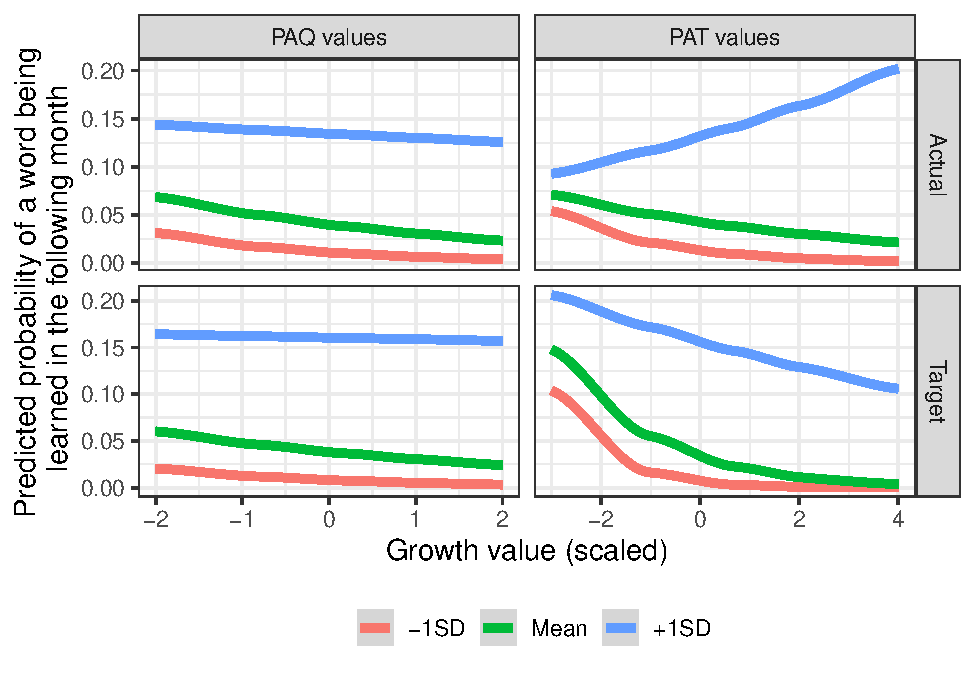
\includegraphics{PhonNetworksProj_files/figure-latex/figure-plot-slopes-1.pdf}
\caption{\label{fig:figure-plot-slopes}Interaction plot showing effect of Age * PAT/PAQ growth value interaction on predicted learning outcomes in both Target and Actual data (French data only). Lines show mean AoP (z-scored) and +/- 1SD around the mean. PAT/PAQ values are z-scored.}
\end{figure}

All outcomes from the simple slopes analyses are shown in Table \ref{tab:table-all-slopes}. Looking first at the English data, more frequent words were acquired predictably at all three time-points, and the effect of word frequency increased with age in both Actual and Target data. The Age x Frequency interaction was significant in the Target data only, while shorter words were more likely to be acquired across all three time-points; this tendency diminished over time.

Looking now at the French data, word length and both PAT and PAQ values interacted with age in both Actual and Target data. Shorter words tended to be acquired earlier, and this effect diminished with age, to the extent that the slope taken at the later time-point was not significant, in both Actual and Target data. Turning to predictions set out in H2, analysis of the Age x PAT interaction did not support this: only the earlier slope shows a significant interaction, whereby words with \emph{lower} PAT values were more likely to be acquired in early development in both Actual and Target data. This trend diminishes with age, such that later slopes are no longer significant in the Actual data, and the extent of the effect is smaller in the Target data, though still negative, and still significant at the mean time-point. The trends were similar for PAQ values: words with lower PAQ values were acquired earlier, and later slopes did not show a significant effect, in both Actual and Target data.

\hypertarget{data-type-comparisons}{%
\subsubsection{Data type comparisons}\label{data-type-comparisons}}

In H3, it was predicted that systematicity would be stronger in Actual, compared to Target, data. We would therefore expect PAT values to be higher (indicating more connectivity) in Actual data at each time-point. This analysis only applies to PAT, given that PAQ values do not change month-by-month, and that the global network is generated from Target forms anyway.

To test this hypothesis, a linear mixed-effects regression model was run using the \emph{lmerTest} package in R (Kuznetsova, Brockhoff, \& Christensen, 2017). For each word, data was only included for the month before the word's age of production, such that PAT values indicated connectivity in the learned month, rather than all of the potential months in which the word could have first been produced. The model included PAT growth values as the dependent variable and Data type, Word length, Word frequency and Age as fixed effects. Word length and Word frequency were both qualified with an interaction with Age; subject was included as a random effect with a by-subject random slope included for the effect of Age. French and English data were modeled separately. Likelihood ratio tests comparing models with and without the effect of Data type included revealed a significant difference between the full and the null models (English: \(\chi^2 (1)\)=11.60, \emph{p}=.001; French: (\(\chi^2 (1)\)=269.07, \emph{p}=\textless{} .001). In support of H3, in both cases PAT values for the Actual data were significantly higher than those of the Target data (English: \emph{b}=-0.06, \emph{p}=.001; French: \emph{b}=-0.93, \emph{p}=\textless{} .001).

\hypertarget{simulated-networks-1}{%
\subsection{Simulated Networks}\label{simulated-networks-1}}

Finally, network graphs generated from the Target and Actual data of each corpus were compared to simulated small world and random networks of equivalent size to determine whether the data (the \emph{Real} networks) differed from the \emph{Simulated} networks. Recall that PAT-like network growth should reflect a small-world network growth structure. Two key components of small-world networks were compared: mean path length and clustering coefficient. PAT-like network growth (recall that small world networks cannot tell us anything about PAQ-like growth) typically has a low mean path length and a high clustering coefficient; we would expect the Real data to differ significantly from the Simulated Erdős--Rényi network, and to see no statistical difference between the Real network and the Simulated Watts-Strogatz network. Below, the two measures will be discussed in turn, for Target and Actual data from each corpus.

\hypertarget{mean-path-length}{%
\subsubsection{Mean Path Length}\label{mean-path-length}}

Mean path length was calculated for each child's monthly networks using the \emph{igraph()} package in R (Csardi \& Nepusz, 2006). For both Target and Actual data, an equivalent-sized Watts-Strogatz network was generated, and a single Erdős--Rényi network. Watts-Strogatz simulations match both the mean degree and the network size of each network in each month, and so two separate networks were generated for Target and Actual data to reflect the different properties of each. Erdős--Rényi networks require only network size to be specified - as this is constant across Target and Actual data, only one such network was generated per month. Mixed effects linear regression models were generated for each corpus, with mean path length as the dependent variable, a Data type (Real-Target, Real-Actual, Watts-Strogatz-Target, Watts-Strogatz-Actual and Erdős--Rényi) x Age interaction included as a fixed effect, and Subject as a random effect. Age was initially included as a by-Subject random slope, but the model would not converge and so this was removed.

Model comparisons with both English and French data revealed a significant main effect for Data type (English: \(\chi^2 (8)\)=411.09, \emph{p} \textless{} .001; French: \(\chi^2 (8)\)=456.21, \emph{p} \textless{} .001). Follow-up models were run for each corpus on only Target/Actual data (Real Target vs.~Simulated Target vs.~Erdős--Rényi, and Real Actual vs.~Simulated Actual vs.~Erdős--Rényi) to establish differences between the Real and Simulated data. See Figure \ref{fig:Figure-path-length}.

\begin{figure}
\centering
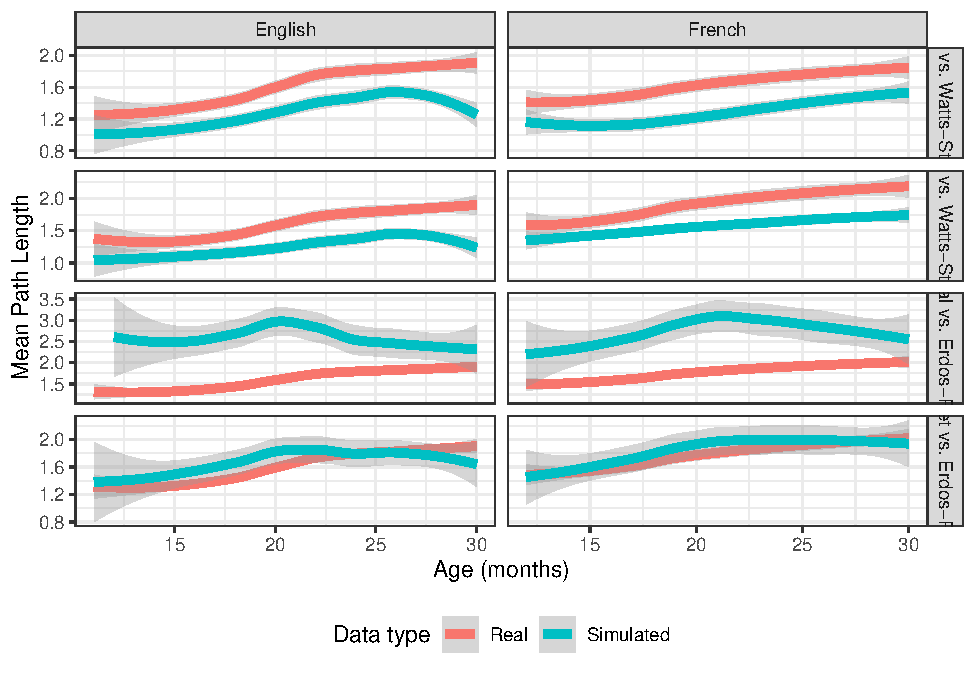
\includegraphics{PhonNetworksProj_files/figure-latex/Figure-path-length-1.pdf}
\caption{\label{fig:Figure-path-length}Change in mean path length over time, in Real data (Actual or Target) compared with Watts-Strogatz and Erdos-Renyi simulations representing small-world and random network growth properties, respectively. Coloured lines represent Data type; grey bands represent 95\% CIs.}
\end{figure}

\begin{longtable}[t]{cccccccccc}
\caption{\label{tab:table-pathlength}Outputs from linear regression models testing the effect of Real and Simulated data on path length. English and French data, both Actual and Target.}\\
\toprule
\multicolumn{2}{c}{ } & \multicolumn{4}{c}{Actual} & \multicolumn{4}{c}{Target} \\
\cmidrule(l{3pt}r{3pt}){3-6} \cmidrule(l{3pt}r{3pt}){7-10}
Effect & Corpus & beta & SE & t & p & beta & SE & t & p\\
\midrule
Intercept & English & 0.78 & 0.23 & 3.418 & 0.00 & 3.47 & 0.26 & 13.475 & 0.00\\
Real vs. Erdos Renyi & English & 2.72 & 0.34 & 7.949 & 0.00 & -2.66 & 0.34 & -7.770 & 0.00\\
Real vs. Watts-Strogatz & English & -0.06 & 0.32 & -0.192 & 0.85 & -2.68 & 0.34 & -7.773 & 0.00\\
Age & English & 0.04 & 0.01 & 4.008 & 0.00 & -0.04 & 0.01 & -3.331 & 0.00\\
Erdos Renyi x Age & English & -0.08 & 0.01 & -5.231 & 0.00 & 0.08 & 0.01 & 5.018 & 0.00\\
\addlinespace
Watts-Strogatz x Age & English & -0.01 & 0.01 & -0.860 & 0.39 & 0.06 & 0.02 & 3.929 & 0.00\\
Intercept & French & 1.04 & 0.19 & 5.556 & 0.00 & 3.47 & 0.26 & 13.475 & 0.00\\
Real vs. Erdos Renyi & French & 2.05 & 0.29 & 7.165 & 0.00 & -2.66 & 0.34 & -7.770 & 0.00\\
Real vs. Watts-Strogatz & French & -0.32 & 0.26 & -1.219 & 0.22 & -2.68 & 0.34 & -7.773 & 0.00\\
Age & French & 0.03 & 0.01 & 3.388 & 0.00 & -0.04 & 0.01 & -3.331 & 0.00\\
\addlinespace
Erdos Renyi x Age & French & -0.04 & 0.01 & -3.016 & 0.00 & 0.08 & 0.01 & 5.018 & 0.00\\
Watts-Strogatz x Age & French & 0.00 & 0.01 & -0.140 & 0.89 & 0.06 & 0.02 & 3.929 & 0.00\\
\bottomrule
\end{longtable}

For both Actual and Target data in both corpora, the Real data differed significantly from the random Erdős--Rényi network, as predicted. See Table \ref{tab:table-pathlength}. Again as predicted, in both cases the Actual data did not differ from the Simulated Watts-Strogatz model, though the opposite was true for the Target data. These outcomes are consistent with predictions in H3.

\begin{figure}
\centering
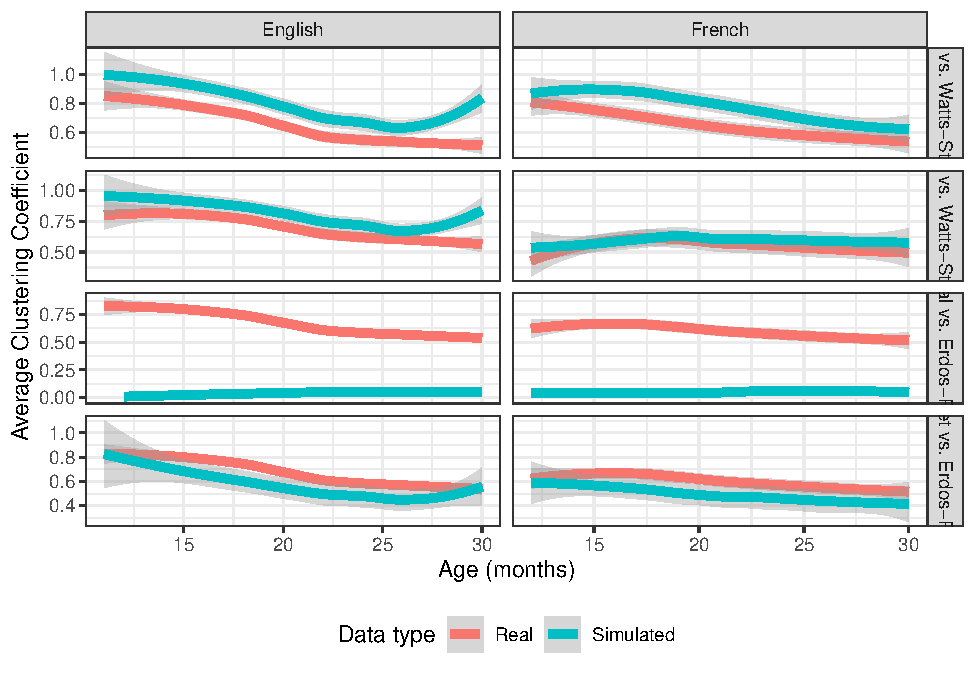
\includegraphics{PhonNetworksProj_files/figure-latex/Figure-clust-coef-1.pdf}
\caption{\label{fig:Figure-clust-coef}Change in mean clustering coefficient over time, in Real data (Actual or Target) compared with Watts-Strogatz and Erdos-Renyi simulations representing small-world and random network growth properties, respectively. Coloured lines represent Data type; grey bands represent 95\% CIs.}
\end{figure}

\hypertarget{clustering-coefficient}{%
\subsection{Clustering Coefficient}\label{clustering-coefficient}}

Similarly, average clustering coefficient was calculated for each child's monthly networks using the \emph{igraph()} package, for both the Real and Simulated data. As Figure \ref{fig:Figure-clust-coef} shows, in both corpora, this variable was lower in the Simulated data than the Real data, in both Target and Actual forms. As above, mixed effects linear regression models were generated for each corpus; the same model structure was used, but this time with average clustering coefficient as the dependent variable.

Again model comparisons revealed a significant main effect for Data type (English: \(\chi^2 (8)\)=869.16, \emph{p} \textless{} .001; French: \(\chi^2 (8)\)=456.21, \emph{p} \textless{} .001).

\begin{longtable}[t]{cccccccccc}
\caption{\label{tab:table-clust}Outputs from linear regression models testing the effect of Real and Simulated data on mean clustering coefficient. English and French data, both Actual and Target.}\\
\toprule
\multicolumn{2}{c}{ } & \multicolumn{4}{c}{Actual} & \multicolumn{4}{c}{Target} \\
\cmidrule(l{3pt}r{3pt}){3-6} \cmidrule(l{3pt}r{3pt}){7-10}
Effect & Corpus & beta & SE & t & p & beta & SE & t & p\\
\midrule
Intercept & English & 1.09 & 0.05 & 22.054 & 0.00 & 0.06 & 0.06 & 1.050 & 0.30\\
Real vs. Erdos Renyi & English & -1.05 & 0.07 & -15.387 & 0.00 & 1.04 & 0.07 & 15.540 & 0.00\\
Real vs. Watts-Strogatz & English & 0.09 & 0.06 & 1.371 & 0.17 & 1.10 & 0.07 & 16.368 & 0.00\\
Age & English & -0.02 & 0.00 & -10.415 & 0.00 & 0.00 & 0.00 & -0.190 & 0.85\\
Erdos Renyi x Age & English & 0.02 & 0.00 & 7.168 & 0.00 & -0.02 & 0.00 & -6.263 & 0.00\\
\addlinespace
Watts-Strogatz x Age & English & 0.00 & 0.00 & 0.809 & 0.42 & -0.02 & 0.00 & -5.490 & 0.00\\
\midrule
Intercept & French & 0.98 & 0.05 & 20.037 & 0.00 & 0.06 & 0.06 & 1.050 & 0.30\\
Real vs. Erdos Renyi & French & -0.88 & 0.06 & -15.358 & 0.00 & 1.04 & 0.07 & 15.540 & 0.00\\
Real vs. Watts-Strogatz & French & 0.18 & 0.05 & 3.508 & 0.00 & 1.10 & 0.07 & 16.368 & 0.00\\
Age & French & -0.02 & 0.00 & -9.471 & 0.00 & 0.00 & 0.00 & -0.190 & 0.85\\
\addlinespace
Erdos Renyi x Age & French & 0.01 & 0.00 & 5.377 & 0.00 & -0.02 & 0.00 & -6.263 & 0.00\\
Watts-Strogatz x Age & French & 0.00 & 0.00 & -1.082 & 0.28 & -0.02 & 0.00 & -5.490 & 0.00\\
\bottomrule
\end{longtable}

Model outputs are shown in Table \ref{tab:table-clust}. Again, across both corpora the Real (Actual and Target) data differed significantly from the random Erdős--Rényi network. However, this time only the Actual data in the English corpus showed no difference between the Real and the Simulated Watts-Strogatz data; in the French data, this was marginally significant. Again, this lends support (albeit partial in this case) to H3.

\hypertarget{discussion}{%
\section{Discussion}\label{discussion}}

This study tested two established frameworks of network growth in the context of early phonological development: preferential attachment (PAT) and preferential acquisition (PAQ) (Fourtassi et al., 2020; Hills et al., 2009; Siew \& Vitevitch, 2020). Using naturalistic data to quantify infants' actual productions of word forms, it was possible to establish similarity (or connectedness) across the phonological properties of infants' early words, and map how this changes over time. Based on previous analyses showing that infants' early productions tend to share phonological and prosodic properties (e.g.~Vihman, 2016; Waterson, 1971; see also Vihman \& Keren-Portnoy, 2013), it was hypothesised that the early vocabulary would grow in a PAT-like manner (H1) -- that is, should constitute dense clusters of similar-sounding forms -- and that acquisition should be most systematic earlier on in development (H2). Expanding on two key studies in this area (Fourtassi et al., 2020; Siew \& Vitevitch, 2020), it was also predicted that a network consisting of infants' actual productions (that is, the child's \emph{realization} of the target forms) should demonstrate more typical PAT-like growth than an equivalent network constituting just the target forms (H3).

Two of these predictions were supported by the data. First, in support of H1, while network growth models showed evidence for both PAT- and PAQ-like growth, this was consistently more strongly in favour of PAT. That is, in a given month, infants tended to produce words that connected to more densely-connected words in the existing network. Overall, newly-acquired words were produced in a similar way to existing words in the network, such that they form dense clusters of similar-sounding forms. While PAT was a better predictor of acquisition, PAQ also significantly predicted word learning (alongside PAT) in the English Actual and French Target data. This is consistent with previous findings showing that PAT and PAQ are not necessarily mutually exclusive models of network growth (Amatuni \& Bergelson, 2017; Fourtassi et al., 2020; Siew \& Vitevitch, 2020).

Second, in support of H3, PAT-like growth was more convincing for the Actual than the Target data: nested model comparisons revealed that data type (Actual versus Target) accounted for significant variance in PAT values, whereby Target data had significantly lower PAT values than Actual data. In the English data, PAT values were 6\% lower in the Target data on average, and in the French data this difference was substantial, with 88\% lower Target PAT values. This reveals that infants' Actual phonological networks develop in a more systematic way than we would expect from looking only at Target forms.

The analysis of small-world network properties partially supported these two hypotheses. When compared with simulated small-world networks (Watts-Strogatz models), Actual -- but not Target -- data resembled a prototypical PAT-like network in the English corpus; that is, there was no statistical difference between the Actual data and the simulated PAT-like model. In the French corpus the results were less clear, but still showed partial support for PAT-like network growth in the Actual data. In both corpora, Target data differed significantly from the prototypical PAT-like network. Given that this component of the analysis cannot be extended to include an analysis of PAQ, direct comparisons between PAT and PAQ cannot be made, but results suggest PAT-like growth in the Actual data over and above the Target data.

Hypothesis 2 predicted that PAT-like network growth would be stronger in earlier development, based on previous analyses that show infants' earliest words to be phonologically similar (e.g.~Deuchar \& Quay, 2000). However, results were inconsistent: the English corpus showed no interaction between age and PAT values, and in the French corpus earlier-acquired words tended to have \emph{lower} PAT values in both Target and Actual data. Results for PAQ were similarly inconsistent: the French Target data showed that earlier-acquired words had lower PAQ values, while in the English Actual data higher PAQ values predicted earlier acquisition. These differential results could reflect the complexities of between-child analyses, where each child may approach the acquisition process in a slightly different way. A larger sample size may allow more holistic generalizations to be made about changes over time; connectivity across the nine networks differed in this data, and these differences may not be corpus- or language-specific, but may reflect the variability expected across early language development.

The present analysis sheds new light on systematicity in early language acquisition, specifically regarding the role of PAT- and PAQ-like models of phonological development. Previous studies have drawn on age of acquisition data, using the target form as the index of production (Fourtassi et al., 2020; Siew \& Vitevitch, 2020). This has allowed study of vocabulary growth across a large sample, and findings have presented a new perspective on the role of phonological neighbourhoods in early acquisition. However, these analyses have not interrogated the role of \emph{production}. By considering networks in relation to \emph{the way infants produce} their early-acquired words, it has been possible to consider network growth in early acquisition from a novel perspective. The findings presented here reveal a systematic approach to early phonological development, as infants exploit their existing production capacity to produce new words with familiar articulatory routines. These results support many previous studies that show lexical development to take place via the implementation of systematic structures and templates (Vihman, 2019; Vihman \& Keren-Portnoy, 2013; Waterson, 1971), and also model a new way of analysing phonological systematicity in infants' early productions, which can be extended to larger samples and applied to a wider variety of languages.

Given that Fourtassi and colleagues (2020) analysed data from children of similar ages using the same subset of words (i.e.~CDI words), we would expect the current findings to map on to their results, particularly in the analysis of Target data. However, this is not the case: their study reveals consistently stronger evidence for PAQ. This may reflect direct differences in the type of data used: in the present study, the order of acquisition (and thereby the model of network growth) reflects the chronological order of individual children's production in naturalistic data. On the other hand, month-by-month acquisition norms taken from thousands of children's CDIs model an \enquote{average} order of acquisition, whereby words that \emph{tend to} appear earlier in the developing lexicon are biased towards an earlier age of acquisition. Frank and colleagues ({\textbf{???}}) report the first 10 words of infants acquiring American English, which (for stop consonants only) contain two instances of /m/, three each of /n/ and /d/, five /b/ and one /g/. In naturalistic production, however, a word's phonological form may prime the acquisition of other similar-sounding words: production of \emph{baby} may be shortly followed by other \emph{bib} and \emph{ball} (cf.~McCune \& Vihman, 2001), while in vocabulary norms, acquisition of \emph{baby}, \emph{bib} and \emph{ball} is represented at the group level. Vocabulary norming data thus represents an \enquote{averaging out} of phonological connectedness across thousands of infants, making it strongly biased towards PAQ-like growth. Previous similar studies perhaps represent a more general, one-size-fits-all trajectory to lexical development, whereas these results capture individual clusters of connectivity as children acquire words that match the phonological characteristics of existing words in the lexicon.

Indeed, studies of infants' early words show that, on a word-by-word basis, early-acquired forms tend to consist of the same set of consonants, in both target and actual forms. This reflects the child's \enquote{selection} of early words to match their own consonant repertoire (McCune \& Vihman, 2001; Stoel-Gammon \& Cooper, 1984; Vihman, 2019). Given that these results show evidence for PAT-like growth in both Actual (English) and Target (English and French) data, it appears that infants are selectively acquiring forms that match their own production preferences, and are either producing these forms accurately (\emph{selected}, in Vihman's terms) or \emph{adapting} them to match their preferred output patterns. Within Vihman's framework, phonological development involves the selection or adaption of lexical units to fit a set of easily-accessible articulatory categories. That is, an infant systematically acts upon new understanding (i.e.~acquired receptive vocabulary items) within the limitations of their development, selecting existing categories to deal with challenges presented in production. These are \enquote{well-worn paths} that represent the stable and well-rehearsed production routines that drive selection, and later adaption, of infants' early word forms.

Note that evidence was also found for PAQ-like acquisition, specifically in the French data. This is consistent with previous studies that show a combined role for both PAT and PAQ growth models in lexical (both phonological and semantic) development (Amatuni \& Bergelson, 2017; Fourtassi et al., 2020). Amatuni and Bergelson (2017) propose that PAT and PAQ could work together in development, such that PAQ may \enquote{{[}supplement{]} PAT by providing a structured sampling space for new word selection} (p.5). That is, a combination of PAT and PAQ would provide both internal (output-driven) and external (input-driven) roles in development. Given that acquisition is a dynamic and interactive process (Thelen \& Smith, 1996), with ample evidence showing the effects of the input on early word learning (Ambridge, Kidd, Rowland, \& Theakston, 2015; Rowe, 2012), it is to be expected that both models would be at work simultaneously during acquisition.

This study raises new questions for future analyses into systematicity in phonological development. While efforts were made to fully characterise the phonological content of infants' early productions -- through using distinctive features with Euclidean, rather than Levenshtein, distance, and observing Actual productions alongside Target forms -- still it was not possible to capture the full extent of systematicity, i.e.~the presence of prosodic structures or templates. Future work in this area should expand the analyses to consider the development and systematic implementation of templates. Furthermore, given that analyses of two languages revealed differing results, it would be valuable to extend the approach to yet more languages. Systematicity has been demonstrated across languages (Khattab \& Al-Tamimi, 2013; Szreder, 2013; Vihman \& Vihman, 2011), and so it should be possible to find cross-linguistic commonalities in network growth. Indeed, differences across languages would raise questions about the cognitive reality of systematicity in phonological development. Finally, the regression models included only two additional factors of acquisition -- word length and frequency. To fully encompass the nature of early acquisition, it would be necessary to index additional factors such as word class (given that all word classes on the CDI were included in the analysis) and vocabulary size, both of which are known to affect phonological development (Braginsky, Yurovsky, Marchman, \& Frank, 2019; Jones, Cabiddu, Andrews, \& Rowland, 2021).

\hypertarget{conclusion}{%
\section{Conclusion}\label{conclusion}}

This works shows that when naturalistic data is considered within a networks account, we find stronger evidence for PAT-like network growth over PAQ-like growth in both English and French data. English-learning infants acquired words that would connect to the most highly-connected nodes in the existing network (PAT-like growth), whereas in the earliest stages of development French infants preferred words that were less likely to connect to highly-connected nodes. When we look at the target form of the words infants acquire and how they produce them, in both cases we see evidence to show that early acquisition is driven -- at least in part -- by preferences in the output. That is, infants acquire words that cluster together phonologically, and produce them systematically such that early production represents clusters of similar-sounding forms.

\newpage

\hypertarget{references}{%
\section{References}\label{references}}

\begingroup
\setlength{\parindent}{-0.5in}
\setlength{\leftskip}{0.5in}

\hypertarget{refs}{}
\leavevmode\hypertarget{ref-amaral_classes_2011}{}%
Amaral, L. A. N., Scala, A., Barthelemy, M., \& Stanley, H. E. (2011). Classes of small-world networks. In \emph{The structure and dynamics of networks} (pp. 207--210). Princeton, NJ: Princeton University Press.

\leavevmode\hypertarget{ref-amatuni_semantic_2017}{}%
Amatuni, A., \& Bergelson, E. (2017). \emph{Semantic networks generated from early linguistic input} (preprint). Animal Behavior; Cognition. \url{https://doi.org/10.1101/157701}

\leavevmode\hypertarget{ref-ambridge_ubiquity_2015}{}%
Ambridge, B., Kidd, E., Rowland, C. F., \& Theakston, A. L. (2015). The ubiquity of frequency effects in first language acquisition*. \emph{Journal of Child Language}, \emph{42}(2), 239--273. \url{https://doi.org/10.1017/S030500091400049X}

\leavevmode\hypertarget{ref-bell_network_2017}{}%
Bell, M., Perera, S., Piraveenan, M., Bliemer, M., Latty, T., \& Reid, C. (2017). Network growth models: A behavioural basis for attachment proportional to fitness. \emph{Scientific Reports}, \emph{7}(1), 42431. \url{https://doi.org/10.1038/srep42431}

\leavevmode\hypertarget{ref-de_boysson-bardies_adaptation_1991}{}%
Boysson-Bardies, B. de, \& Vihman, M. M. (1991). Adaptation to language: Evidence from babbling and first words in four languages. \emph{Language}, \emph{67}(2), 297--319. \url{https://doi.org/10.2307/415108}

\leavevmode\hypertarget{ref-braginsky_consistency_2019}{}%
Braginsky, M., Yurovsky, D., Marchman, V. A., \& Frank, M. C. (2019). Consistency and variability in children's word learning across languages. \emph{Open Mind: Discoveries in Cognitive Science}, \emph{3}, 52--67.

\leavevmode\hypertarget{ref-chomsky_noam_sound_1968}{}%
Chomsky, Noam, \& Halle, Morris. (1968). \emph{The sound pattern of english}. New York, NY: Harper; Rowe.

\leavevmode\hypertarget{ref-R-igraph}{}%
Csardi, G., \& Nepusz, T. (2006). The igraph software package for complex network research. \emph{InterJournal}, \emph{Complex Systems}, 1695. Retrieved from \url{http://igraph.org}

\leavevmode\hypertarget{ref-demuth_word-minimality_2006}{}%
Demuth, K., Culbertson, J., \& Alter, J. (2006). Word-minimality, epenthesis and coda licensing in the early acquisition of english. \emph{Language and Speech}, \emph{49}(2), 137--174.

\leavevmode\hypertarget{ref-demuth_katherine_prosodically-conditioned_2008}{}%
Demuth, K., \& Tremblay, A. (2008). Prosodically-conditioned variability in children's production of french determiners. \emph{Journal of Child Language}, \emph{35}(1). Retrieved from \url{https://www-cambridge-org.abc.cardiff.ac.uk/core/journals/journal-of-child-language/article/prosodicallyconditioned-variability-in-childrens-production-of-french-determiners/B34D994A1EA63DFF841D1C2C7974D6FE}

\leavevmode\hypertarget{ref-deuchar_bilingual_2000}{}%
Deuchar, M., \& Quay, S. (2000). \emph{Bilingual acquisition: Theoretical implications of a case study}. Oxford, UK: Oxford University Press.

\leavevmode\hypertarget{ref-fenson_variability_1994}{}%
Fenson, L., Dale, P. S., Reznick, J. S., Bates, E., Thal, D. J., Pethick, M., Stephen J. Tomasello, \ldots{} Stiles, J. (1994). Variability in early communicative development. \emph{Monographs of the Society for Research in Child Development}, \emph{59}. \url{https://doi.org/10.2307/1166093}

\leavevmode\hypertarget{ref-ferguson_words_1975}{}%
Ferguson, C. A., \& Farwell, C. B. (1975). Words \& sounds in early language acquisition. \emph{Language}, \emph{51}, 419--439.

\leavevmode\hypertarget{ref-fourtassi_growth_2020}{}%
Fourtassi, A., Bian, Y., \& Frank, M. C. (2020). The growth of children's semantic and phonological networks: Insight from 10 languages. \emph{Cognitive Science}, \emph{44}(7), e12847. \url{https://doi.org/10.1111/cogs.12847}

\leavevmode\hypertarget{ref-frank_wordbank_2017}{}%
Frank, M. C., Braginsky, M., Yurovsky, D., \& Marchman, V. A. (2017). Wordbank: An open repository for developmental vocabulary data. \emph{Journal of Child Language}, \emph{44}(3), 677--694. \url{https://doi.org/10.1017/S0305000916000209}

\leavevmode\hypertarget{ref-hedlund_gregory_phon_2020}{}%
Hedlund, G., \& Rose, Y. (2020). \emph{Phon 3.1 {[}computer software{]}}. Retrieved from \url{https://phon.ca}

\leavevmode\hypertarget{ref-hills_longitudinal_2009}{}%
Hills, T. T., Maouene, M., Maouene, J., Sheya, A., \& Smith, L. (2009). Longitudinal analysis of early semantic networks preferential attachment or preferential acquisition? \emph{Psychological Science}, \emph{20}(6), 729--739. \url{https://doi.org/10.1111/j.1467-9280.2009.02365.x}

\leavevmode\hypertarget{ref-jones_chunks_2021}{}%
Jones, G., Cabiddu, F., Andrews, M., \& Rowland, C. (2021). Chunks of phonological knowledge play a significant role in children's word learning and explain effects of neighborhood size, phonotactic probability, word frequency and word length. \emph{Journal of Memory and Language}, \emph{119}, 104232. \url{https://doi.org/10.1016/j.jml.2021.104232}

\leavevmode\hypertarget{ref-jones_children_2019}{}%
Jones, S. D., \& Brandt, S. (2019). Do children really acquire dense neighbourhoods? \emph{Journal of Child Language}, \emph{46}(6), 1260--1273. \url{https://doi.org/10.1017/S0305000919000473}

\leavevmode\hypertarget{ref-kern_sophie_ifdc_2010}{}%
Kern, S., \& Gayraud, F. (2010). \emph{IFDC}. Grenoble: Les éditions la cigale.

\leavevmode\hypertarget{ref-khattab_influence_2013}{}%
Khattab, G., \& Al-Tamimi, J. (2013). Influence of geminate structure on early arabic templatic patterns. In M. M. Vihman \& T. Keren-Portnoy (Eds.), \emph{The emergence of phonology: Whole-word approaches and cross-linguistic evidence} (pp. 374--414). Cambridge: Cambridge University Press. \url{https://doi.org/10.1017/CBO9780511980503.018}

\leavevmode\hypertarget{ref-kuznetsova_lmertest_2017}{}%
Kuznetsova, A., Brockhoff, P. B., \& Christensen, R. H. B. (2017). \{lmerTest\} package: Tests in linear mixed effects models. \emph{Journal of Statistical Software}, \emph{82}(13), 1--26. \url{https://doi.org/10.18637/jss.v082.i13}

\leavevmode\hypertarget{ref-macwhinney_childes_2000}{}%
MacWhinney, B. (2000). \emph{The CHILDES project: Tools for analyzing talk} (3rd ed.). Mahwah, NJ: Lawrence Erlbaum Associates. \url{https://doi.org/10.1177/026565909200800211}

\leavevmode\hypertarget{ref-mccune_early_2001}{}%
McCune, L., \& Vihman, M. M. (2001). Early phonetic and lexical development. \emph{Journal of Speech, Language, and Hearing Research}, \emph{44}(3), 670--684. \url{https://doi.org/10.1044/1092-4388(2001/054)}

\leavevmode\hypertarget{ref-mcleod_childrens_2018}{}%
McLeod, S., \& Crowe, K. (2018). Children's consonant acquisition in 27 languages: A cross-linguistic review. \emph{American Journal of Speech-Language Pathology}, 1--26. \url{https://doi.org/10.1044/2018_AJSLP-17-0100}

\leavevmode\hypertarget{ref-monaghan_measures_2010}{}%
Monaghan, P., Christiansen, M. H., Farmer, T. A., \& Fitneva, S. A. (2010). Measures of phonological typicality. \emph{The Mental Lexicon}, \emph{5}(3), 281--299. \url{https://doi.org/10.1075/ml.5.3.02mon}

\leavevmode\hypertarget{ref-R-base}{}%
R Core Team. (2020). \emph{R: A language and environment for statistical computing}. Vienna, Austria: R Foundation for Statistical Computing. Retrieved from \url{https://www.R-project.org/}

\leavevmode\hypertarget{ref-rowe_longitudinal_2012}{}%
Rowe, M. L. (2012). A longitudinal investigation of the role of quantity and quality of child-directed speech in vocabulary development. \emph{Child Development}, \emph{83}(5), 1762--1774. \url{https://doi.org/10.1111/j.1467-8624.2012.01805.x}

\leavevmode\hypertarget{ref-seidenberg_dyslexia_1999}{}%
Seidenberg, M. S., Harm, M. W., \& Seidenberg, M. S. (1999). Dyslexia: Insights from connectionist models. \emph{Unpublished Doctoral Dissertation, University of Southern California, Los}, 491--528.

\leavevmode\hypertarget{ref-siew_investigation_2020}{}%
Siew, C. S. Q., \& Vitevitch, M. S. (2020). An investigation of network growth principles in the phonological language network. \emph{Journal of Experimental Psychology: General}. \url{https://doi.org/10.1037/xge0000876}

\leavevmode\hypertarget{ref-steyvers_large-scale_2005-2}{}%
Steyvers, M., \& Tenenbaum, J. B. (2005a). The large-scale structure of semantic networks: Statistical analyses and a model of semantic growth. \emph{Cognitive Science}, \emph{29}(1), 41--78. \url{https://doi.org/10.1207/s15516709cog2901_3}

\leavevmode\hypertarget{ref-steyvers_large-scale_2005}{}%
Steyvers, M., \& Tenenbaum, J. B. (2005b). The large-scale structure of semantic networks: Statistical analyses and a model of semantic growth. \emph{Cognitive Science}, \emph{29}(1), 41--78. \url{https://doi.org/10.1207/s15516709cog2901_3}

\leavevmode\hypertarget{ref-stoel-gammon_patterns_1984}{}%
Stoel-Gammon, C., \& Cooper, J. A. (1984). Patterns of early lexical and phonological development. \emph{Journal of Child Language}, \emph{11}(2), 247--271. \url{https://doi.org/10.1017/S0305000900005766}

\leavevmode\hypertarget{ref-szreder_acquisition_2013}{}%
Szreder, M. (2013). The acquisition of consonant clusters in polish: A case study. In M. M. Vihman \& T. Keren-Portnoy (Eds.), \emph{The emergence of phonology: Whole-word approaches and cross-linguistic evidence} (pp. 343--361). Cambridge: Cambridge University Press. \url{https://doi.org/10.1017/CBO9780511980503.016}

\leavevmode\hypertarget{ref-thelen_esther_dynamic_1996}{}%
Thelen, E., \& Smith, L. (1996). \emph{A dynamic systems approach to the development of cognition and action.} Boston, MA: MIT Press.

\leavevmode\hypertarget{ref-vihman_prosodic_2016}{}%
Vihman, M. (2016). Prosodic structures and templates in bilingual phonological development. \emph{Bilingualism: Language and Cognition}, \emph{19}(1), 69--88. \url{https://doi.org/10.1017/S1366728914000790}

\leavevmode\hypertarget{ref-vihman_variable_1993}{}%
Vihman, M. M. (1993). Variable paths to early word production. \emph{Journal of Phonetics}, \emph{21}, 61--82.

\leavevmode\hypertarget{ref-vihman_phonological_2014}{}%
Vihman, M. M. (2014). \emph{Phonological development: The first two years} (2nd ed.). Malden, MA: Wiley-Blackwell.

\leavevmode\hypertarget{ref-vihman_phonological_2019}{}%
Vihman, M. M. (2019). \emph{Phonological templates in development}. Oxford, UK: Oxford University Press.

\leavevmode\hypertarget{ref-vihman_external_1994}{}%
Vihman, M. M., Kay, E., Boysson-Bardies, B. de, Durand, C., \& Sundberg, U. (1994). External sources of individual differences? A cross-linguistic analysis of the phonetics of mothers' speech to 1-year-old children. \emph{Developmental Psychology}, \emph{30}(5), 651--662.

\leavevmode\hypertarget{ref-vihman_emergence_2013}{}%
Vihman, M. M., \& Keren-Portnoy, T. (2013). The emergence of phonology: Whole-word approaches, cross-linguistic evidence. In M. M. Vihman \& T. Keren-Portnoy (Eds.), \emph{The emergence of phonology: Whole-word approaches and cross-linguistic evidence}. Cambridge: Cambridge University Press. \url{https://doi.org/10.1017/CBO9780511980503.002}

\leavevmode\hypertarget{ref-arnon_first_2011}{}%
Vihman, M., \& Vihman, V.-A. (2011). From first words to segments: A case study in phonological development. In I. Arnon \& E. V. Clark (Eds.), \emph{Trends in language acquisition research} (Vol. 7, pp. 109--134). Amsterdam: John Benjamins Publishing Company. \url{https://doi.org/10.1075/tilar.7.07vih}

\leavevmode\hypertarget{ref-waterson_child_1971}{}%
Waterson, N. (1971). Child phonology : A prosodic view. \emph{Journal of Linguistics}, \emph{7}(2), 179--211. \url{https://doi.org/10.1017/S0022226700002917}

\leavevmode\hypertarget{ref-watts_collective_1998}{}%
Watts, D. J., \& Strogatz, S. H. (1998). Collective dynamics of ``small-world'' networks, \emph{393}, 3.

\textbackslash end\{longtable\}
\endgroup


\end{document}
